\documentclass[10pt]{beamer}

\usepackage{packages}
\title{Exercício Programa 3}
\subtitle{Simulador de sistema de arquivos}
\institute{IME-USP}
\author{Lucas Paiolla Forastiere, 11221911\\ Marcos Siolin Martins, 11221709}
\date{07 de dezembro de 2020}

\begin{document}
    \maketitle
    \section{Sobre o simulador}
    \begin{frame}{Detalhes de Implementação - o sistema de arquivos}
        \begin{itemize}
            \justifying
            \item A representação do sistema de arquivos é armazenada em um arquivo que sempre ocupa \texttt{100MB} no sistema de arquivos real. Caso seja executado \texttt{mount} sobre um arquivo que não exista, será gerado um novo arquivo com \texttt{100MB} onde estará armazenado o \texttt{Bitmap}, a \textt{FAT} e o diretório \texttt{root} (/);
            \item Consideramos que conteúdo de arquivos contém apenas caracteres que ocupam 1 \texttt{byte} em seus nomes e conteúdos, ou seja, que pertencem à tabela \texttt{ASCII}. Isso nos permite controlar quanto espaço cada arquivo ou diretório ocupa;
        \end{itemize}
    \end{frame}
    \begin{frame}{Detalhes de Implementação - o sistema de arquivos}
        \begin{itemize}
            \justifying
            \item Utilizamos o caractere \texttt{|} (pipe) como separador para indicar situações como o fim de nome de arquivo ou fim de conteúdo, então é importante que não existam arquivos que contenham esse caractere no nome ou em seu conteúdo;
            \item Para preencher espaços em branco utilizamos a constante \texttt{CHAR\_NULO} que é um \texttt{' '} (whitespace).
            \item Após dar mount no arquivo que guarda o sistema de arquivos simulado, o conteúdo do arquivo é trazido para memória e as alterações são feitas em memória. As alterações serão gravados no arquivo em disco quando o comando umount for dado.
        \end{itemize}
    \end{frame}
    \begin{frame}{Detalhes de Implementação - o bitmap}
        \begin{itemize}
            \justifying
            \item O Bitmap é implementado como um vetor booleano de tamanho \texttt{NUM\_BLOCOS}, que é a constante que guarda a quantidade de blocos disponíveis para o sistema de arquivos simulado, desconsiderando os blocos necessários para armazenar o Bitmap e a FAT. O valor \texttt{1/true} indica que o bloco está livre e o valor \texttt{0/false} indica que o bloco está ocupado.
            \item O Bitmap ocupa os primeiros 7 blocos do sistema de arquivos simulado, pois precisa armazenar \texttt{NUM\_BLOCOS bytes}. O espaço restante no 7º bloco é desperdiçado;
        \end{itemize}
    \end{frame}
    \begin{frame}{Detalhes de Implementação - a FAT}
        \begin{itemize}
            \justifying
            \item A FAT é implementada como um vetor de inteiros de tamanho \texttt{NUM\_BLOCOS}. O valor em \texttt{ponteiro[i]} indica qual é o próximo bloco após o $i$ na lista ligada do arquivo. Caso esse valor seja igual à \texttt{BLOCO\_NULO} (um valor de um bloco que não existe), então o bloco $i$ é o último na sequência da lista ligada.
            \item Para armazenar esses ponteiros os convertemos para uma string com tamanho fixo $5$, assim, se \texttt{ponteiro[i] = 1}, no sistema de arquivos simulado será armazenado como \texttt{00001}.
            \item A FAT é armazenada nos 32 blocos conseguintes ao Bitmap, pois precisa armazenar \texttt{NUM\_BLOCOS*5 bytes}. O espaço restante no 32º bloco é desperdiçado;
        \end{itemize}
    \end{frame}
    \begin{frame}{Detalhes de Implementação - o root}
        \begin{itemize}
            \justifying
            \item O diretório \texttt{/} é um diretório especial. Ele está sempre ocupando o bloco 0 (a partir de agora desconsideraremos os blocos necessário para armazenar o bitmap e a FAT) e também armazena os próprios metadados, nessa ordem:
            \begin{itemize}
                \justifying
                \item Tempo Criado - ocupa 10 bytes. É a quantidade em segundos devolvida por \texttt{time(NULL)} no momento de criação do arquivo;
                \item Tempo Modificado - ocupa 10 bytes. É a quantidade em segundos devolvida por \texttt{time(NULL)} no momento de última modificação do arquivo;
                \item Tempo Acesso - ocupa 10 bytes. É a quantidade em segundos devolvida por \texttt{time(NULL)} no momento de último acesso do arquivo;
                \item Nome - ocupa x bytes. Ao fim do nome estará o caractere \texttt{'|'}.
            \end{itemize}
        \end{itemize}
    \end{frame}
    \begin{frame}{Detalhes de Implementação - os diretórios}
        \begin{itemize}
            \justifying
            \item Os diretórios armazenam os metadados dos subdiretórios e dos arquivos que estão ``imediatamente abaixo'' do diretório. Os metadados são armazenados na seguinte ordem:
            \begin{itemize}
                \justifying
                \item Ponteiro para o nome - ocupa 8 bytes. Aponta para o endereço do disco onde está o nome do arquivo/diretório;
                \item Diretório - ocupa 1 byte. Indica se os metadados são de um diretório ou de um arquivo;
                \item Número do primeiro bloco - ocupa 5 bytes. Aponta para o primeiro bloco onde o arquivo/diretório está armazenado; 
                \item Tempo Criado - ocupa 10 bytes;
                \item Tempo Modificado - ocupa 10 bytes;
                \item Tempo Acesso - ocupa 10 bytes;                
            \end{itemize}
        \end{itemize}        
    \end{frame}
    \begin{frame}{Detalhes de Implementação - os diretórios}
        \begin{itemize}
            \justifying
            \begin{itemize}
                \justifying
                \item Tamanho - ocupa 8 bytes. Se os metadados são de um diretório, então esse valor é sempre 0;
                \item Nome* - ocupa x bytes. Ao fim do nome estará o caractere \texttt{'|'}.
            \end{itemize}
            \item Os diretórios seguem a estratégia apresentada em aula onde cada subarquivo/subdiretório tem um campo de metadados, com exceção do nome (*), de tamanho fixo e o metadado nome fica armazenado em uma região especial chamada de heap. No campo de metadados existe um ponteiro para o lugar onde o nome está armazenado;
            \item Na nossa implementação a heap está armazenada imediatamente após acabarem todos os campos para os metadados. O começo da heap é indicado pelo caractere \texttt{'|'}.
        \end{itemize}
    \end{frame}
    \begin{frame}{Detalhes de Implementação - os arquivos}
        \begin{itemize}
            \justifying
            \item Quando um arquivo é criado, o espaço necessário para armazenar o conteúdo dele é alocado. Em seguida, alocamos espaço para armazenar os metadados dele no diretório. Caso alguma dessas operações não seja possível, qualquer espaço alocado é liberado e uma mensagem de erro informa que o arquivo não pôde ser salvo;
            \item O fim do conteúdo do arquivo é marcado por um caractere \texttt{'|'}, então é importante que esse caractere não esteja dentro do conteúdo do arquivo. Além disso, assumimos que o conteúdo do arquivo é composto apenas por caracteres \texttt{ASCII}, pois estes ocupam apenas 1 \texttt{byte}, então não o conteúdo do arquivo também não pode conter caracteres que não pertençam à tabela \texttt{ASCII}.
        \end{itemize}
    \end{frame}
    \begin{frame}{Detalhes de Implementação - os comandos}
        \centering
        \begin{table}
            \begin{tabular}{|c|c|c|c|c|}
                \hline
                Comandos & Acesso & Modificação & Criação & Onde \\
                \hline
                \texttt{cp} & X & X & & P \\
                \hline
                \texttt{mkdir} & X & X & & P \\
                \hline
                \texttt{rmdir} & X & X & & P \\
                \hline
                \texttt{cat} &  &  & &  \\
                \hline
                \texttt{touch} & X & X & & AP \\
                \hline
                \texttt{rm} & X & X & & P \\
                \hline
                \texttt{ls} &  &  & &  \\
                \hline
                \texttt{find} &  &  & &  \\
                \hline
            \end{tabular}
            \caption{Tabela indicando o comportamento dos comandos em relação à alteração de tempo dos arquivos.} \label{tabela}
        \end{table}
    \end{frame}
    \begin{frame}{Detalhes de Implementação - os comandos}
        \begin{itemize}
            \justifying
            \item Na tabela \ref{tabela}, a letra \texttt{'A'} na coluna \texttt{'Onde'} significa que as alterações são no próprio arquivo onde foi aplicado o comando e a letra \texttt{'P'} significa que as alterações são no diretório pai;
            \item Quando o comando \texttt{touch} cria um arquivo novo ele muda os tempos no pai, mas quando não, muda apenas o seu próprio tempo de acesso e modificação;
            \item Todos os comandos que criam arquivos atualizam o estado dos três tempos para o arquivo recém-criado.
        \end{itemize}
    \end{frame}
    \begin{frame}{Detalhes de Implementação - os comandos}
        \begin{itemize}
            \justifying
            \item No comando \texttt{df}...;
            \item No comando \texttt{find}... ;
            \item No comando \texttt{rmdir}... (O rmdir não mostra os caminhos deletados, só o nome dos arquivos);
        \end{itemize}
    \end{frame}
    \section{Experimentos}
    \begin{frame}{Experimentos - Sistema de arquivos vazio}
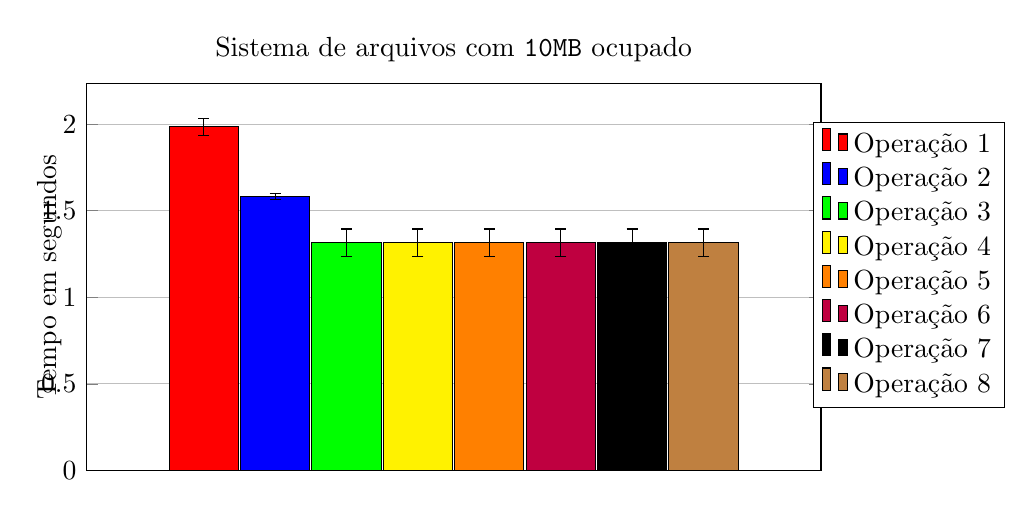
\begin{tikzpicture}
                \begin{axis}[
                        width  = 0.9*\textwidth,
                        height = 6.5cm,
                        major x tick style = transparent,
                        ybar=2*\pgflinewidth,
                        bar width=25pt,
                        ymajorgrids = true,
                        symbolic x coords={Sistema de arquivos com \texttt{10MB} ocupado},
                        xtick = data,
                        xticklabel pos=right,
                        scaled y ticks = false,
                        enlarge x limits=0.50,
                        ymin=0,
                        ylabel={Tempo em segundos},
                        ylabel style={yshift=-0.5cm},
                        legend cell align=left,
                        % legend pos=north east,
                        legend style={at={(1.12,0.9)},anchor=north},
                    ]

                    \addplot[style={fill=red},
                    error bars/.cd,
                    y dir=both,
                    y explicit]
                    coordinates {
                        (Sistema de arquivos com \texttt{10MB} ocupado, 1.985) += (0,0.049) -= (0,0.049)
                    };

                    \addplot[style={fill=blue},
                    error bars/.cd,
                    y dir=both,
                    y explicit]
                    coordinates {
                        (Sistema de arquivos com \texttt{10MB} ocupado, 1.583) += (0,0.016) -= (0,0.016)
                    };

                    \addplot[style={fill=green},
                    error bars/.cd,
                    y dir=both,
                    y explicit]
                    coordinates {
                        (Sistema de arquivos com \texttt{10MB} ocupado, 1.316) += (0,0.0787) -= (0,0.0787)
                    };
                    
                    \addplot[style={fill=yellow},
                    error bars/.cd,
                    y dir=both,
                    y explicit]
                    coordinates {
                        (Sistema de arquivos com \texttt{10MB} ocupado, 1.316) += (0,0.0787) -= (0,0.0787)
                    };

                    \addplot[style={fill=orange},
                    error bars/.cd,
                    y dir=both,
                    y explicit]
                    coordinates {
                        (Sistema de arquivos com \texttt{10MB} ocupado, 1.316) += (0,0.0787) -= (0,0.0787)
                    };
                    \addplot[style={fill=purple},
                    error bars/.cd,
                    y dir=both,
                    y explicit]
                    coordinates {
                        (Sistema de arquivos com \texttt{10MB} ocupado, 1.316) += (0,0.0787) -= (0,0.0787)
                    };
                    \addplot[style={fill=black},
                    error bars/.cd,
                    y dir=both,
                    y explicit]
                    coordinates {
                        (Sistema de arquivos com \texttt{10MB} ocupado, 1.316) += (0,0.0787) -= (0,0.0787)
                    };
                    \addplot[style={fill=brown},
                    error bars/.cd,
                    y dir=both,
                    y explicit]
                    coordinates {
                        (Sistema de arquivos com \texttt{10MB} ocupado, 1.316) += (0,0.0787) -= (0,0.0787)
                    };

                \legend{Operação 1, Operação 2, Operação 3, Operação 4, Operação 5, Operação 6, Operação 7, Operação 8}
                \end{axis}
            \end{tikzpicture}
    \end{frame}
    \begin{frame}{Experimentos - Sistema de arquivos com \texttt{10MB} ocupado}
        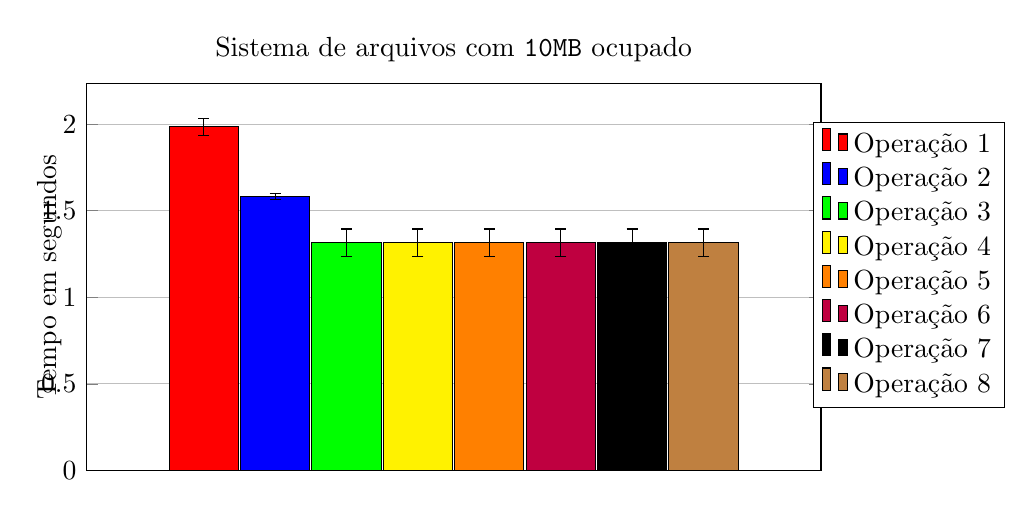
\begin{tikzpicture}
                \begin{axis}[
                        width  = 0.9*\textwidth,
                        height = 6.5cm,
                        major x tick style = transparent,
                        ybar=2*\pgflinewidth,
                        bar width=25pt,
                        ymajorgrids = true,
                        symbolic x coords={Sistema de arquivos com \texttt{10MB} ocupado},
                        xtick = data,
                        xticklabel pos=right,
                        scaled y ticks = false,
                        enlarge x limits=0.50,
                        ymin=0,
                        ylabel={Tempo em segundos},
                        ylabel style={yshift=-0.5cm},
                        legend cell align=left,
                        % legend pos=north east,
                        legend style={at={(1.12,0.9)},anchor=north},
                    ]

                    \addplot[style={fill=red},
                    error bars/.cd,
                    y dir=both,
                    y explicit]
                    coordinates {
                        (Sistema de arquivos com \texttt{10MB} ocupado, 1.985) += (0,0.049) -= (0,0.049)
                    };

                    \addplot[style={fill=blue},
                    error bars/.cd,
                    y dir=both,
                    y explicit]
                    coordinates {
                        (Sistema de arquivos com \texttt{10MB} ocupado, 1.583) += (0,0.016) -= (0,0.016)
                    };

                    \addplot[style={fill=green},
                    error bars/.cd,
                    y dir=both,
                    y explicit]
                    coordinates {
                        (Sistema de arquivos com \texttt{10MB} ocupado, 1.316) += (0,0.0787) -= (0,0.0787)
                    };
                    
                    \addplot[style={fill=yellow},
                    error bars/.cd,
                    y dir=both,
                    y explicit]
                    coordinates {
                        (Sistema de arquivos com \texttt{10MB} ocupado, 1.316) += (0,0.0787) -= (0,0.0787)
                    };

                    \addplot[style={fill=orange},
                    error bars/.cd,
                    y dir=both,
                    y explicit]
                    coordinates {
                        (Sistema de arquivos com \texttt{10MB} ocupado, 1.316) += (0,0.0787) -= (0,0.0787)
                    };
                    \addplot[style={fill=purple},
                    error bars/.cd,
                    y dir=both,
                    y explicit]
                    coordinates {
                        (Sistema de arquivos com \texttt{10MB} ocupado, 1.316) += (0,0.0787) -= (0,0.0787)
                    };
                    \addplot[style={fill=black},
                    error bars/.cd,
                    y dir=both,
                    y explicit]
                    coordinates {
                        (Sistema de arquivos com \texttt{10MB} ocupado, 1.316) += (0,0.0787) -= (0,0.0787)
                    };
                    \addplot[style={fill=brown},
                    error bars/.cd,
                    y dir=both,
                    y explicit]
                    coordinates {
                        (Sistema de arquivos com \texttt{10MB} ocupado, 1.316) += (0,0.0787) -= (0,0.0787)
                    };

                \legend{Operação 1, Operação 2, Operação 3, Operação 4, Operação 5, Operação 6, Operação 7, Operação 8}
                \end{axis}
            \end{tikzpicture}
    \end{frame}
    \begin{frame}{Experimentos - Sistema de arquivos com \texttt{50MB} ocupado}
        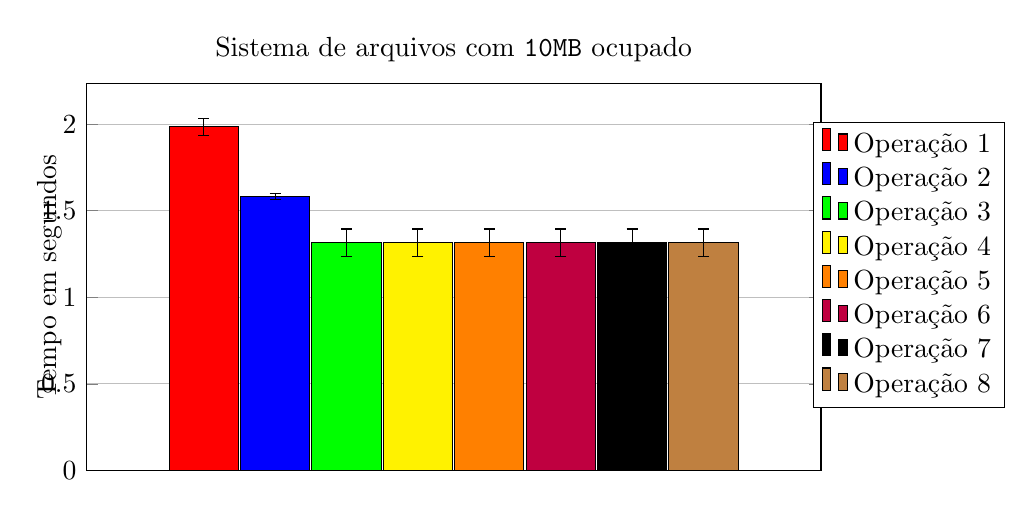
\begin{tikzpicture}
                \begin{axis}[
                        width  = 0.9*\textwidth,
                        height = 6.5cm,
                        major x tick style = transparent,
                        ybar=2*\pgflinewidth,
                        bar width=25pt,
                        ymajorgrids = true,
                        symbolic x coords={Sistema de arquivos com \texttt{10MB} ocupado},
                        xtick = data,
                        xticklabel pos=right,
                        scaled y ticks = false,
                        enlarge x limits=0.50,
                        ymin=0,
                        ylabel={Tempo em segundos},
                        ylabel style={yshift=-0.5cm},
                        legend cell align=left,
                        % legend pos=north east,
                        legend style={at={(1.12,0.9)},anchor=north},
                    ]

                    \addplot[style={fill=red},
                    error bars/.cd,
                    y dir=both,
                    y explicit]
                    coordinates {
                        (Sistema de arquivos com \texttt{10MB} ocupado, 1.985) += (0,0.049) -= (0,0.049)
                    };

                    \addplot[style={fill=blue},
                    error bars/.cd,
                    y dir=both,
                    y explicit]
                    coordinates {
                        (Sistema de arquivos com \texttt{10MB} ocupado, 1.583) += (0,0.016) -= (0,0.016)
                    };

                    \addplot[style={fill=green},
                    error bars/.cd,
                    y dir=both,
                    y explicit]
                    coordinates {
                        (Sistema de arquivos com \texttt{10MB} ocupado, 1.316) += (0,0.0787) -= (0,0.0787)
                    };
                    
                    \addplot[style={fill=yellow},
                    error bars/.cd,
                    y dir=both,
                    y explicit]
                    coordinates {
                        (Sistema de arquivos com \texttt{10MB} ocupado, 1.316) += (0,0.0787) -= (0,0.0787)
                    };

                    \addplot[style={fill=orange},
                    error bars/.cd,
                    y dir=both,
                    y explicit]
                    coordinates {
                        (Sistema de arquivos com \texttt{10MB} ocupado, 1.316) += (0,0.0787) -= (0,0.0787)
                    };
                    \addplot[style={fill=purple},
                    error bars/.cd,
                    y dir=both,
                    y explicit]
                    coordinates {
                        (Sistema de arquivos com \texttt{10MB} ocupado, 1.316) += (0,0.0787) -= (0,0.0787)
                    };
                    \addplot[style={fill=black},
                    error bars/.cd,
                    y dir=both,
                    y explicit]
                    coordinates {
                        (Sistema de arquivos com \texttt{10MB} ocupado, 1.316) += (0,0.0787) -= (0,0.0787)
                    };
                    \addplot[style={fill=brown},
                    error bars/.cd,
                    y dir=both,
                    y explicit]
                    coordinates {
                        (Sistema de arquivos com \texttt{10MB} ocupado, 1.316) += (0,0.0787) -= (0,0.0787)
                    };

                \legend{Operação 1, Operação 2, Operação 3, Operação 4, Operação 5, Operação 6, Operação 7, Operação 8}
                \end{axis}
            \end{tikzpicture}
    \end{frame}

    \begin{frame}{Experimentos - Especificações do SO}

    \end{frame}

    \begin{frame}{Conclusões - Tempo}
    \end{frame}
    \begin{frame}
        \centering
        {\huge Obrigado!}

        $\\$

        Lucas e Marcos

    \end{frame}
\end{document}
